% !TeX program = lualatex


% Do not surround the equal signs with spaces, it causes errors!
\documentclass[
	ruledheaders=section,
	class=report,
	thesis={type=bachelor},
	accentcolor=1c,
	custommargins=true,
	marginpar=false,
	%BCOR = 5mm, % Bindekorrektur
	parskip=half-,
	fontsize=11pt,
	instbox=false
]{tudapub}

% Include preamble to not clutter this file.
% Core packages.
% Primary: English, Secondary: German.
\usepackage[main = english, ngerman]{babel}
% Other packages.
%\usepackage{graphicx}
\usepackage{tikz}
\usepackage{mathtools}
\usepackage{amssymb}
\usepackage{siunitx}
\usepackage{amsthm}
% Remove dot at the end: nopostdot; Don't skip any groups: nogroupskip
\usepackage[xindy, section = section, nonumberlist, sanitize={symbol=false}, shortcuts, acronym, nomain, nowarn]{glossaries}
\usepackage{tabularx}
\usepackage{booktabs}
\usepackage{longtable}
\usepackage{enumitem}
%\usepackage{listings}
\usepackage{xcolor}
\usepackage{caption}
\usepackage{subcaption}
\usepackage{epstopdf}
\usepackage{wrapfig}
\usepackage[ruled, vlined, linesnumbered, resetcount, algochapter]{algorithm2e}
\usepackage[autostyle]{csquotes}
\usepackage{microtype}
\usepackage{physics}
\usepackage{cancel}
\usepackage{hyperref}
\usepackage{tabto}
\usepackage{eqparbox}
\usepackage{pgfplots}
\usepackage{multicol}
\usepackage{listings}
\usepackage{xspace}
\usepackage[bottom]{footmisc}

\usetikzlibrary{arrows.meta, shapes, backgrounds, angles, calc, chains, scopes, decorations.pathmorphing, patterns, positioning, quotes}

% Debug packages.
\usepackage{comment}
\usepackage{todonotes}

% Acronyms.
% Common-language acronyms.
\newacronym{eg}{e.g.}{for example}
\newacronym{ie}{i.e.}{that is}
\newacronym{iid}{i.i.d.}{independently and identically distributed}
\newacronym{wrt}{w.r.t.}{with respect to}
% 2 letters without plural.
\newacronym{em}{EM}{Expectation-Maximization}
\newacronym{gd}{GD}{Gradient Descent}
\newacronym{kl}{KL}{Kullback-Leibler}
% 2 letters with plural.
\newacronym[shortplural = {UTs}, longplural = {Unscented Transformations}]{ut}{UT}{Unscented Transformation}
% 3 letters without plural.
\newacronym{ekf}{EKF}{Extended Kalman Filter}
\newacronym{rts}{RTS}{Rauch-Tung-Striebel}
% 3 letters with plural.
\newacronym[shortplural = {HMMs}, longplural = {Hidden Markov Models}]{hmm}{HMM}{Hidden Markov Model}
\newacronym[shortplural = {LQGs}, longplural = {Linear Quadratic Gaussian}]{lqg}{LQG}{Linear Quadratic Gaussian}
\newacronym[shortplural = {LQRs}, longplural = {Linear Quadratic Regulators}]{lqr}{LQR}{Linear Quadratic Regulator}
\newacronym[shortplural = {ODEs}, longplural = {Ordinal Differential Equations}]{ode}{ODE}{Ordinary Differential Equation}
\newacronym[shortplural = {PDEs}, longplural = {Partial Differential Equations}]{pde}{PDE}{Partial Differential Equation}
\newacronym[shortplural = {VAEs}, longplural = {Variational Auto-Encoders}]{vae}{VAE}{Variational Auto-Encoder}
% 4 letterd without plural.
\newacronym{aevb}{AEVB}{Auto-Encoding Variational Bayes}
% 4 letters with plural.
\newacronym[shortplural = {ELBOs}, longplural = {Evidence Lower Bounds}]{elbo}{ELBO}{Evidence Lower Bound}
\newacronym[shortplural = {LGDSs}, longplural = {Linear Gaussian Dynamical Systems}]{lgds}{LGDS}{Linear Gaussian Dynamical System}

% Operators.
\newglossary[opg]{operator}{opi}{opo}{List of Operators}
\newglossaryentry{expectation}{
	sort		= { expectation value },
	name		= { \ensuremath{\E} },
	symbol		= { \ensuremath{\E[\cdot]} },
	description	= { Expectation value. },
	type		= operator
}
\newglossaryentry{covariance}{
	sort		= { covariance },
	name		= { \ensuremath{\Cov} },
	symbol		= { \ensuremath{\Cov[\cdot]} },
	description	= { Covariance. },
	type		= operator
}
\newglossaryentry{log}{
	sort		= { logarithm },
	name		= { \ensuremath{\log_k} },
	symbol		= { \ensuremath{\log_k(\cdot)} },
	description	= { Logarithm of base \ensuremath{k}. If no base is given, the natural logarithm. },
	type		= operator
}
\newglossaryentry{trace}{
	sort		= { linalg trace },
	name		= { \ensuremath{\tr} },
	symbol		= { \ensuremath{\tr(\cdot)} },
	description	= { Trace of a matrix. },
	type		= operator
}
\newglossaryentry{diag}{
	sort		= { linalg diag },
	name		= { \ensuremath{\diag} },
	symbol		= { \ensuremath{\diag(\alpha_1, \alpha_2, \cdots, \alpha_n)} },
	description	= { Represents a \(n\)-dimensional diagonal matrix with diagonal entries \(\alpha_i\), \( i = 1, 2, \cdots, n \). },
	type		= operator
}
\newglossaryentry{src}{
	sort		= { cubature spherical-radial },
	name		= { \ensuremath{\SRC} },
	symbol		= { \ensuremath{\SRC[\vec{f}; \vec{\mu}, \mat{\Sigma}]} },
	description	= { Evaluation of spherical-radical cubature rule of function \(\vec{f}\) under mean \(\vec{\mu}\) and covariance \(\mat{\Sigma}\). },
	type		= operator
}

% Symbols.
\newglossary[syg]{symbol}{sys}{syo}{List of Symbols}
\newglossaryentry{theta}{
	sort		= { parameters theta },
	name		= { \ensuremath{\vec{\theta}} },
	description	= { Vector of parameters from a probability distribution, a model or similar. },
	type		= symbol
}
\newglossaryentry{gaussian}{
	sort		= { distribution gaussian },
	name		= { \ensuremath{\mathcal{N}(\vec{\mu}, \mat{\Sigma})} },
	description	= { Multivariate normal probability distribution with mean \(\vec{\mu}\) and covariance \(\mat{\Sigma}\). },
	type		= symbol
}


\makeglossaries

% Tikz-diagrams for not cluttering the text.

\newcommand{\tikzHarmonicOscillator}{
	\begin{tikzpicture}
		\node [draw, rectangle] (m) at (0, 3) {\(m\)};
		\draw [thick] (-1.5, 5) -- (1.5, 5);
		\fill [pattern = north east lines] (-1.5, 5) rectangle (1.5, 5.2);
		\draw [decoration = { aspect = 0.3, segment length = 2mm, amplitude = 3mm, coil }, decorate] (0, 5) -- node[left, xshift = -0.4cm]{\(k\)} (m);

		\coordinate (xA) at (1, 4.5);
		\coordinate (xB) at (1, 3.5);
		\draw [->] (xA) -- node[right]{\(x\)} (xB);
	\end{tikzpicture}
}

\newcommand{\tikzSimplePendulum}{
	\begin{tikzpicture}
		\node [draw, circle, fill, minimum width = 0.5cm] (C) at (0, 0) {};
		\node [draw, circle] (mass) at (90-30:3cm) {\(m\)};
		\coordinate (A) at (90:3cm);
		\draw (C) -- coordinate(cm) (mass);
		\path (cm) -- node[right]{\(\ell_1\)} (mass);
		\draw [dashed] (C) -- (A);
		\draw pic [draw, "$\varphi$", angle radius = 1.5cm, angle eccentricity = 0.85] {angle=mass--C--A};

		\draw [<-] (-0.5, 1) -- node[left]{\(g\)} (-0.5, 2);
	\end{tikzpicture}
}

\newcommand{\tikzDoublePendulum}{
	\begin{tikzpicture}
		\def\L{3};
		\node [draw, circle, fill, minimum width = 0.5cm] (C) at (0, 0) {};
		\node [draw, circle] (mass1) at (270+20:\L) {\(m_{\mathclap{\,\,1}}\)};
		\coordinate (A) at (270:\L);
		\draw (C) -- coordinate(cm1) (mass1);
		\path (cm1) -- node[right]{\(\ell_1\)} (mass1);
		\draw [dashed] (C) -- (A);
		\draw pic [draw, "$\,\varphi_1$", angle radius = 1.5cm, angle eccentricity = 0.85] {angle=A--C--mass1};

		\draw [<-] (-0.5, -2) -- node[left]{\(g\)} (-0.5, -1);

		\begin{scope}[rotate=300, shift=(mass1)]
			\coordinate (B) at (0:\L);
			\node [draw, circle] (mass2) at (30:\L) {\(m_{\mathclap{\,\;2}}\)};
			\draw (mass1) -- coordinate(cm2) (mass2);
			\path (cm2) -- node[right, yshift = 2pt]{\(\ell_2\)} (mass2);
			\draw [dashed] (mass1) -- (B);
			\draw pic [draw, "$\,\varphi_2$", angle radius = 1.5cm, angle eccentricity = 0.85] {angle=B--mass1--mass2};
		\end{scope}
	\end{tikzpicture}
}

\newcommand{\tikzCartpole}{
	\begin{tikzpicture}
		\coordinate (cartTopLeft);
		\draw [fill] (cartTopLeft) rectangle coordinate(C) ++(1.5, 0.5);
		\coordinate [above = 3 of C] (A);
		\draw [dashed] (C) -- (A);
		\coordinate [left = 4 of C] (a);
		\coordinate [right = 4 of C] (b);
		\draw (a) -- (b);

		\draw [<-] (0.25, 1.5) -- node[left]{\(g\)} (0.25, 2.5);

		\coordinate [below = 0.5 of C] (xInd);
		\coordinate [above = 0.1 of xInd] (xIndA);
		\coordinate [below = 0.1 of xInd] (xIndB);
		\draw (xIndA) -- (xIndB);
		\coordinate [right = 0.75 of xInd] (xInd2);
		\draw [->] (xInd) -- node[below, xshift = -1pt]{\(x\)} (xInd2);

		\begin{scope}[shift=(C)]
			\coordinate (mass) at (90-30:3);
			\draw [line width = 1mm] (C) -- coordinate(cm) (mass);
			\path (cm) -- node[right, yshift=-2pt]{\(L\)} (mass);
			\draw pic [draw, "$\theta$", angle radius = 1.5cm, angle eccentricity = 0.85] {angle=mass--C--A};
		\end{scope}
	\end{tikzpicture}
}

\newcommand{\tikzKoopmanOperator}{
	\begin{tikzpicture}[->, state/.style = { draw, circle, minimum width = 1cm, minimum height = 1cm }]
		\node [state]                  (y1) {\raisebox{-5pt}{\(\vec{y}_{\,\mathclap{\,1}}\)}};
		\node [state, right = 1 of y1] (y2) {\raisebox{-5pt}{\(\vec{y}_{\,\mathclap{\,2}}\)}};
		\node [state, right = 1 of y2] (y3) {\raisebox{-5pt}{\(\vec{y}_{\,\mathclap{\,3}}\)}};
		\node [minimum width = 1cm, minimum height = 1cm, right = 1 of y3] (yD) {\(\cdots\)};
		\node [state, right = 1 of yD] (yT) {\raisebox{-5pt}{\(\vec{y}_{\,\mathclap{\,T}}\)}};

		\node [state, below = 1 of y1] (x1) {\raisebox{-5pt}{\(\vec{x}_{\,\mathclap{\,1}}\)}};
		\node [state, below = 1 of y2] (x2) {\raisebox{-5pt}{\(\vec{x}_{\,\mathclap{\,2}}\)}};
		\node [state, below = 1 of y3] (x3) {\raisebox{-5pt}{\(\vec{x}_{\,\mathclap{\,3}}\)}};
		\node [minimum width = 1cm, minimum height = 1cm, below = 1 of yD] (xD) {\(\cdots\)};
		\node [state, below = 1 of yT] (xT) {\raisebox{-5pt}{\(\vec{x}_{\,\mathclap{\,T}}\)}};

		% TikZ centering magic. Align on the states, not the h^{-1} stuff or so. Ensures all three HMM, LGDS and Koopman have the same width.
		\coordinate [left = 0.5 of x1] (needle1);
		\coordinate [right = 0.5 of xT] (needle2);
		\draw [opacity = 0] (needle1) -- (x1);
		\draw [opacity = 0] (needle2) -- (xT);

		\draw (y1) -- node[above]{\(\mathcal{K}\,\)} (y2);
		\draw (y2) -- node[above]{\(\mathcal{K}\,\)} (y3);
		\draw (y3) -- node[above]{\(\mathcal{K}\,\)} (yD);
		\draw (yD) -- node[above]{\(\mathcal{K}\,\)} (yT);

		\draw (x1) -- node[below]{\(\vec{F}\)} (x2);
		\draw (x2) -- node[below]{\(\vec{F}\)} (x3);
		\draw (x3) -- node[below]{\(\vec{F}\)} (xD);
		\draw (xD) -- node[below]{\(\vec{F}\)} (xT);

		\draw (y1) to[bend right = 15] node[left]{\(\vec{h}\)} (x1);
		\draw (y2) to[bend right = 15] node[left]{\(\vec{h}\)} (x2);
		\draw (y3) to[bend right = 15] node[left]{\(\vec{h}\)} (x3);
		\draw (yT) to[bend right = 15] node[left]{\(\vec{h}\)} (xT);

		\draw [dashed] (x1) to[bend right = 15] node[right]{\(\vec{h}^{-1}\)} (y1);
		\draw [dashed] (x2) to[bend right = 15] node[right]{\(\vec{h}^{-1}\)} (y2);
		\draw [dashed] (x3) to[bend right = 15] node[right]{\(\vec{h}^{-1}\)} (y3);
		\draw [dashed] (xT) to[bend right = 15] node[right]{\(\vec{h}^{-1}\)} (yT);
	\end{tikzpicture}
}

\newcommand{\tikzHiddenMarkovModel}{
	\begin{tikzpicture}[->, state/.style = { draw, circle, minimum width = 1cm, minimum height = 1cm }]
		\node [state]                  (s1) {\raisebox{-5pt}{\(s_{\,\mathclap{\,1}}\)}};
		\node [state, right = 1 of s1] (s2) {\raisebox{-5pt}{\(s_{\,\mathclap{\,2}}\)}};
		\node [state, right = 1 of s2] (s3) {\raisebox{-5pt}{\(s_{\,\mathclap{\,3}}\)}};
		\node [minimum width = 1cm, minimum height = 1cm, right = 1 of s3] (sD) {\(\cdots\)};
		\node [state, right = 1 of sD] (sT) {\raisebox{-5pt}{\(s_{\,\mathclap{\,T}}\)}};

		\node [state, below = 1 of s1] (y1) {\raisebox{-5pt}{\(\vec{y}_{\,\mathclap{\,1}}\)}};
		\node [state, below = 1 of s2] (y2) {\raisebox{-5pt}{\(\vec{y}_{\,\mathclap{\,2}}\)}};
		\node [state, below = 1 of s3] (y3) {\raisebox{-5pt}{\(\vec{y}_{\,\mathclap{\,3}}\)}};
		\node [state, below = 1 of sT] (yT) {\raisebox{-5pt}{\(\vec{y}_{\,\mathclap{\,T}}\)}};

		% TikZ centering magic. Align on the states, not the h^{-1} stuff or so. Ensures all three HMM, LGDS and Koopman have the same width.
		\coordinate [left = 0.5 of s1] (needle1);
		\coordinate [right = 0.5 of sT] (needle2);
		\draw [opacity = 0] (needle1) -- (s1);
		\draw [opacity = 0] (needle2) -- (sT);

		\draw (s1) -- (s2);
		\draw (s2) -- (s3);
		\draw (s3) -- (sD);
		\draw (sD) -- (sT);

		\draw (s1) -- (y1);
		\draw (s2) -- (y2);
		\draw (s3) -- (y3);
		\draw (sT) -- (yT);
	\end{tikzpicture}
}

\newcommand{\tikzLinearGaussianDynamicalSystem}{
	\begin{tikzpicture}[->, state/.style = { draw, circle, minimum width = 1cm, minimum height = 1cm }]
		\node [state]                  (x1) {\raisebox{-5pt}{\(\vec{s}_{\,\mathclap{\,1}}\)}};
		\node [state, right = 1 of x1] (x2) {\raisebox{-5pt}{\(\vec{s}_{\,\mathclap{\,2}}\)}};
		\node [state, right = 1 of x2] (x3) {\raisebox{-5pt}{\(\vec{s}_{\,\mathclap{\,3}}\)}};
		\node [minimum width = 1cm, minimum height = 1cm, right = 1 of x3] (xD) {\(\cdots\)};
		\node [state, right = 1 of xD] (xT) {\raisebox{-5pt}{\(\vec{s}_{\,\mathclap{\,T}}\)}};

		\node [state, below = 1 of x1] (y1) {\raisebox{-5pt}{\(\vec{y}_{\,\mathclap{\,1}}\)}};
		\node [state, below = 1 of x2] (y2) {\raisebox{-5pt}{\(\vec{y}_{\,\mathclap{\,2}}\)}};
		\node [state, below = 1 of x3] (y3) {\raisebox{-5pt}{\(\vec{y}_{\,\mathclap{\,3}}\)}};
		\node [state, below = 1 of xT] (yT) {\raisebox{-5pt}{\(\vec{y}_{\,\mathclap{\,T}}\)}};

		% TikZ centering magic. Align on the states, not the h^{-1} stuff or so. Ensures all three HMM, LGDS and Koopman have the same width.
		\coordinate [left = 0.5 of x1] (needle1);
		\coordinate [right = 0.5 of xT] (needle2);
		\draw [opacity = 0] (needle1) -- (x1);
		\draw [opacity = 0] (needle2) -- (xT);

		\draw (x1) -- node[above]{\(\mat{A}\)} (x2);
		\draw (x2) -- node[above]{\(\mat{A}\)} (x3);
		\draw (x3) -- node[above]{\(\mat{A}\)} (xD);
		\draw (xD) -- node[above]{\(\mat{A}\)} (xT);

		\draw (x1) -- node[left]{\(\mat{C}\)} (y1);
		\draw (x2) -- node[left]{\(\mat{C}\)} (y2);
		\draw (x3) -- node[left]{\(\mat{C}\)} (y3);
		\draw (xT) -- node[left]{\(\mat{C}\)} (yT);
	\end{tikzpicture}
}

\newcommand{\tikzNonlinearGaussianKoopman}{
\begin{tikzpicture}[->, state/.style = { draw, circle, minimum width = 1cm, minimum height = 1cm }]
	\node [state]                  (x1) {\raisebox{-5pt}{\(\vec{s}_{\,\mathclap{\,1}}\)}};
	\node [state, right = 1 of x1] (x2) {\raisebox{-5pt}{\(\vec{s}_{\,\mathclap{\,2}}\)}};
	\node [state, right = 1 of x2] (x3) {\raisebox{-5pt}{\(\vec{s}_{\,\mathclap{\,3}}\)}};
	\node [minimum width = 1cm, minimum height = 1cm, right = 1 of x3] (xD) {\(\cdots\)};
	\node [state, right = 1 of xD] (xT) {\raisebox{-5pt}{\(\vec{s}_{\,\mathclap{\,T}}\)}};

	\node [state, below = 1 of x1] (y1) {\raisebox{-5pt}{\(\vec{y}_{\,\mathclap{\,1}}\)}};
	\node [state, below = 1 of x2] (y2) {\raisebox{-5pt}{\(\vec{y}_{\,\mathclap{\,2}}\)}};
	\node [state, below = 1 of x3] (y3) {\raisebox{-5pt}{\(\vec{y}_{\,\mathclap{\,3}}\)}};
	\node [state, below = 1 of xT] (yT) {\raisebox{-5pt}{\(\vec{y}_{\,\mathclap{\,T}}\)}};

	% TikZ centering magic. Align on the states, not the h^{-1} stuff or so. Ensures all three HMM, LGDS and Koopman have the same width.
	\coordinate [left = 0.5 of x1] (needle1);
	\coordinate [right = 0.5 of xT] (needle2);
	\draw [opacity = 0] (needle1) -- (x1);
	\draw [opacity = 0] (needle2) -- (xT);

	\draw (x1) -- node[above]{\(\mat{A}\)} (x2);
	\draw (x2) -- node[above]{\(\mat{A}\)} (x3);
	\draw (x3) -- node[above]{\(\mat{A}\)} (xD);
	\draw (xD) -- node[above]{\(\mat{A}\)} (xT);

	\draw (x1) -- node[left]{\(\vec{g}(\cdot)\)} (y1);
	\draw (x2) -- node[left]{\(\vec{g}(\cdot)\)} (y2);
	\draw (x3) -- node[left]{\(\vec{g}(\cdot)\)} (y3);
	\draw (xT) -- node[left]{\(\vec{g}(\cdot)\)} (yT);
\end{tikzpicture}
}

% #1 := Optional TikZ style arguments.
% #2 := Number of input neurons.
% #3 := Number of hidden neurons.
% #4 := Number of output neurons.
% #5 := Number of hidden layers plus one.
\newcommand{\tikzNeuralNetwork}[5][]{
	\begin{scope}[
				input neuron/.style = { draw, circle, minimum width = 0.2cm, minimum height = 0.2cm, fill = TUDa-4a },
				neuron/.style = { draw, circle, minimum width = 0.2cm, minimum height = 0.2cm, fill = TUDa-1a },
				output neuron/.style = { draw, circle, minimum width = 0.2cm, minimum height = 0.2cm, fill = TUDa-6a },
				#1
			]
		\def\xMultiplier{1}
		\foreach \x in { 0, ..., #5 }
			\ifthenelse{\x = 0}
				{\foreach \y in { 1, ..., #2 }}
				{\ifthenelse{\x = #5}
					{\foreach \y in { 1, ..., #4 }}
					{\foreach \y in { 1, ..., #3 }}}
				\ifthenelse{\x = 0}
					{\node [input neuron] (e\x\y) at (\xMultiplier*\x, \y+#3/2-#2/2) {}}
					{\ifthenelse{\x = #5}
						{\node [output neuron] (e\x\y) at (\xMultiplier*\x, \y+#3/2-#4/2) {}}
						{\node [neuron] (e\x\y) at (\xMultiplier*\x, \y) {}}};
		\foreach \xB [count = \xA from 0] in { 1, ..., #5 }
			\ifthenelse{\xA = 0}
				{\foreach \yA in { 1, ..., #2 }}
				{\foreach \yA in { 1, ..., #3 }}
				\ifthenelse{\xB = #5}
					{\foreach \yB in { 1, ..., #4 }}
					{\foreach \yB in { 1, ..., #3 }}
					\draw (e\xA\yA) -- (e\xB\yB);
		\ifthenelse{#2 > #3}
			{
				\def\m{#2};
				\def\cA{e01};
				\def\cB{e0#2};
			}
			{
				\def\m{#3};
				\def\cA{e11};
				\def\cB{e1#3};
			}
		\ifthenelse{\m > #4}{}{
			\def\cA{e#51};
			\def\cB{e#5#4};
		}
		\path let \p1 = (e01.west), \p2 = (\cA.south) in coordinate (bottom-left) at (\x1, \y2);
		\path let \p1 = (e#51.east), \p2 = (\cB.north) in coordinate (top-right) at (\x1, \y2);
		\path [use as bounding box] (bottom-left) rectangle (top-right);
	\end{scope}
}

% #1 := Optional TikZ style arguments.
% #2 := Observation dimension.
% #3 := Latent dimension.
% #4 := Number of neurons.
% #5 := Number of hidden layers plus one.
\newcommand{\tikzAutoEncoder}[5][]{
	\begin{scope}[#1]
		\tikzNeuralNetwork{#2}{#4}{#3}{#5}
		\tikzNeuralNetwork[input neuron/.style = { draw, circle, minimum width = 0.2cm, minimum height = 0.2cm, fill = TUDa-3a }, xshift = #5cm]{#3}{#4}{#2}{#5}
	\end{scope}
}

\newcommand{\tikzVariationalAutoEncoder}{
	\begin{tikzpicture}
		\tikzAutoEncoder{3}{2}{5}{5}
	\end{tikzpicture}
}

\newcommand{\tikzPredictionFilteringSmoothing}{
	\begin{tikzpicture}
		\coordinate (aStart) at (0, 0);
		\coordinate (bStart) at (0, 1);
		\coordinate (cStart) at (0, 2);
		\coordinate (aEnd) at (10, 0);
		\coordinate (bEnd) at (10, 1);
		\coordinate (cEnd) at (10, 2);
		\coordinate (kA) at (4.5, -0.5);
		\coordinate (kB) at (4.5, 2.5);
		\coordinate (kpA) at (5, -0.5);
		\coordinate (kpB) at (5, 2.5);
		\coordinate (t1) at (0, -0.5);
		\coordinate (tT) at (10, -0.5);

		\foreach \n in { 0, 1, 2 } {
			\foreach \t in { 0, ..., 20 } {
				\ifthenelse{\t = 0 \OR \t = 20}{
					\draw (\t*0.5, \n+0.25) -- (\t*0.5, \n-0.25);
				}{
					\draw (\t*0.5, \n+0.125) -- (\t*0.5, \n-0.125);
				}
			}
		}

		\draw (aStart) -- (aEnd);
		\draw (bStart) -- (bEnd);
		\draw (cStart) -- (cEnd);

		\draw [line width = 1pt, dotted] (kA) -- (kB);
		\draw [line width = 0.75pt] (kpA) -- (kpB);

		\node [right = 0.5 of aEnd] {Smoothing};
		\node [right = 0.5 of bEnd] {Filtering};
		\node [right = 0.5 of cEnd] {Prediction};

		\node [below = 0 of kA] {\small \( t - 1 \)};
		\node [below = 0 of kpA] {\small \( t \)};

		\node [below = 0 of t1] {\( 0 \)};
		\node [below = 0 of tT] {\( T \)};

		\path [fill = black, opacity = 0.1] (0, 0.2) -- (10, 0.2) -- (10, -0.2) -- (0, -0.2) -- cycle;
		\path [fill = black, opacity = 0.1] (0, 1.2) -- (5, 1.2) -- (5, 0.8) -- (0, 0.8) -- cycle;
		\path [fill = black, opacity = 0.1] (0, 2.2) -- (4.5, 2.2) -- (4.5, 1.8) -- (0, 1.8) -- cycle;
	\end{tikzpicture}
}



\begin{document}
	% No page numbering for the preamble.
	\pagenumbering{gobble}

	\Metadata{
		title = Learning Stochastic Nonlinear Dynamics With the Koopman Operator,
		author = Fabian Damken
	}

	\title{Learning Stochastic Nonlinear Dynamics With the Koopman Operator}
	\subtitle{Lernen stochastischer nichtlinearer Systemdynamiken mit dem Koopman-Operator}
	\author{Fabian Damken}
	\birthplace{Frankfurt am Main}
	\reviewer{Jan Peters \and Joe Watson}
	\department{inf}
	\institute{Intelligent Autonomous Systems}
	%\group{Working Group}
	\addTitleBoxLogo*{
\includegraphics[width=0.75\linewidth]{img/iasLogo.pdf}}

	\submissiondate{\today}
	\examdate{\today}

	%\tuprints{urn=1234,printid=12345}
	%\dedication{Für alle, die \TeX{} nutzen.}

	\maketitle

	\affidavit

	\tableofcontents

	\chapter*{Figures~and~Tables}
		\begingroup
		\let\clearpage\relax
		\listoffigures\listoftables
		\endgroup
	% end

	\chapter*{Abbreviations,~Symbols and Operators}
		\glsaddall
		\printglossary[type = acronym, title = List of Abbreviations, style = iasThesisGeneral]
		\printglossary[type = symbol, style = iasThesisGeneral]
		\printglossary[type = operator, style = iasThesisOperators]
	% end

	% Start page numbering.
	\pagenumbering{arabic}

	% Someone wants content, for whatever reason.
	\chapter{Introduction}
	\label{c:introduction}
	\IMRADlabel{introduction}

	\todo{Introduction: Content}
% end

	\chapter{Motivation}
	\label{c:motivation}

	\todo{Motivation: Content}
% end

	\chapter{Foundations}
	\label{c:foundations}
	\IMRADlabel{methods}

	\section{Dynamical Systems}
		A \emph{dynamical system}~\cite{birkhoffDynamicalSystems1927} is a (physical) system that evolves over time \(t\) and is completely defined by the values of \(n\) real variables
		\begin{align*}
			x_1, x_2, \,\cdots\!, x_n \quad\longleftrightarrow\quad \vec{x} = \begin{bmatrix} x_1 & x_2 & \cdots & x_m \end{bmatrix}^T
		\end{align*}
		called the \emph{state} and often written in vector form (right). Given the differentiability of these values, we can also study their rate of change (often referred to as the "velocity") and the rate of change of the rate of change (often referred to as the "acceleration"):
		\begin{align*}
			\dot{\vec{x}} = \dv{\vec{x}}{t} \qquad \ddot{\vec{x}} = \dv[2]{\vec{x}}{t}
		\end{align*}
		Describing these systems is possible using differential equations, both ordinary and partial ones. A general \ac{ode} is given by an implicit equation
		\begin{align}
			\vec{0} = \vec{F}\big( \vec{x}, \vec{x}^{(1)}, \vec{x}^{(2)}, \,\cdots\!, \vec{x}^{(k - 1)}, \vec{x}^{(k)}; t \big),\quad \vec{x}^{(l)} \coloneqq \dv[l]{\vec{x}}{t}  \label{eq:ode}
		\end{align}
		which establishes a connection between the state itself and its time derivatives. We call a function \( \vec{x}(t) \) a \emph{solution} of an \ac{ode} if its derivatives fulfill the given \ac{ode}~\eqref{eq:ode}. We will now employ some definitions and terms that we will use throughout the whole thesis.
		\begin{description}[leftmargin = 3cm]
			\item[Order] If \( \vec{x}^{(k)} \) is the derivative of highest order that appears in the \ac{ode}, the \ac{ode} is called to be of order \(k\).
			\item[Linearity] An \ac{ode} is \emph{linear} if \(\vec{F}\) is a linear function in terms of the state and its derivatives, \ac{ie} it is given as a linear combination
		\end{description}
		\begin{align*}
			\vec{F} = \vec{r}(t) + \sum_{i = 1}^{k} c_i(t) \vec{x}^{(i)},\quad \vec{r}(t) : \R \to \R^n,\, c_i(t) : \R \to \R
		\end{align*}
		\begin{description}[leftmargin = 3cm]
			\item[Autonomous] If \(\vec{F}\) explicitly is independent of \(t\) (\ac{ie} \( \pdv{\vec{F}}{t} = \vec{0} \)), the \ac{ode} is called \emph{autonomous}.
			\item[Homogenity] If no term  of \(\vec{F}\) is independent of the state or its derivatives, the \ac{ode} is called \emph{homogeneous}. For any homogeneous \ac{ode} one of its solutions is the trivial solution \( \vec{x} \equiv \vec{0} \).
		\end{description}

		In all of the following, we assume to have explicit, autonomous, first order \acp{ode}. This is valid because we can transform every explicit higher order \ac{ode} into a system of first order \acp{ode} as well as we can introduce another "time state" which makes our \ac{ode} autonomous.

		The solution theory for linear \acp{ode} is highly evolved and solutions exist for nearly every possible \ac{ode}. But for nonlinear \acp{ode}, the world looks different. With the exception of some rare cases, nonlinear \acp{ode} are not tractable. Hence, we often need approximations for the nonlinear case. Some well-known approaches for these approximations are \ac{eg} \emph{small angle approximation} for Sines and Cosines. In small angle approximations, we Taylor-expand \( \sin \)/\( \cos \) at \( \varphi_a = 0 \) and cut all higher order terms:
		\begin{gather*}
			\sin(\varphi) = \varphi - \underbrace{\frac{\varphi^3}{3!} + \frac{\varphi^5}{5!} + \cdots}_\text{higher order terms} \approx \varphi \\
			\cos(\varphi) = 1 - \underbrace{\frac{\varphi^2}{2!} + \frac{\varphi^4}{4!} - \frac{\varphi^6}{6!} + \cdots}_\text{higher order terms} \approx 1
		\end{gather*}
		This approach is illustrated in~\autoref{fig:smallAngleApproximation}.

		\begin{figure}
			\centering
			\begin{subfigure}[t]{0.5\linewidth}
				\centering
				\includegraphics[width = \linewidth]{figures/introduction/generated/small-angle-approximation-sin.pdf}
				\caption{Small angle approximation \( \sin(\varphi) \approx \varphi \) of Sine.}
			\end{subfigure}%
			~
			\begin{subfigure}[t]{0.5\linewidth}
				\centering
				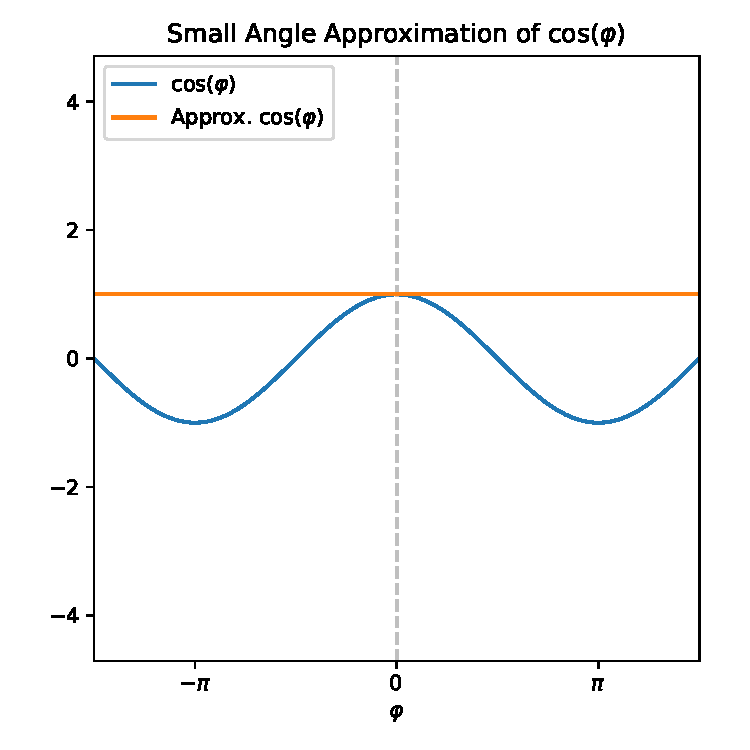
\includegraphics[width = \linewidth]{figures/introduction/generated/small-angle-approximation-cos.pdf}
				\caption{Small angle approximation \( \cos(\varphi) \approx 1 \) of Cosine.}
			\end{subfigure}
			\caption{Visualization of the small angle approximation (given is orange) of the basic trigonometric functions Sine and Cosine (given in blue). It is clear that the approximation is only valid in a small region around zero (\( \varphi \approx 0 \)).}
			\label{fig:smallAngleApproximation}
		\end{figure}

		We now look at two examples of dynamical systems, one which is linear and one that is not.

		\subsection{Harmonic Oscillator}
			\label{subsec:harmonicOscillator}

			\begin{figure}
				\centering
				\tikzHarmonicOscillator
				\caption{Illustration of a simple harmonic oscillator with mass \(m\), spring stiffness \(k\) and position \(x\) that is not affected by any external force like gravity. The mass is in equilibrium if \( x = 0 \).}
				\label{fig:simpleHarmonicOscillator}
			\end{figure}

			The \emph{simple harmonic oscillator} describes the dynamical system of a mass \(m\) that is attached to a spring that is following Hooke's Law with stiffness \(k\) (see~\autoref{fig:simpleHarmonicOscillator}). This harmonic oscillator is described by the \ac{ode}
			\begin{align}
				m\ddot{x} = -kx \quad\iff\quad \ddot{x} = -\frac{k}{m} x  \label{eq:harmonicOscillator}
			\end{align}
			where \(x\) and \(\ddot{x}\) are the position and acceleration of the mass, respectively. Note that if \( x = 0 \), the mass is in equilibrium and no force is acting on it.

			By using basic results in the solution theory of linear \acp{ode}, we see that the general solution is given as
			\begin{align*}
				x(t) = A \cos\Big(t \sqrt{k / m} + \varphi\Big)
			\end{align*}
			with the amplitude \(A\) and the phase \(\varphi\) (see~\autoref{app:harmonicOscillatorSolution} for the derivation of the solution). As neither gravity nor damping or other external forces are involved in the dynamical system, the motion continues forever with a non-changing amplitude.
		% end

		\subsection{Simple Pendulum}
			\label{subsec:simplePendulum}

			\begin{figure}
				\centering
				\tikzSimplePendulum
				\caption{Illustration of an inverse pendulum with mass \(m\) and displacement \(\varphi\) that is only affected by gravity and no other external force. The mass is in equilibrium for both \( \varphi = 0 \) and \( \varphi = \pi \), where the former is an unstable equilibrium.}
				\label{fig:simplePendulum}
			\end{figure}

			The \emph{inverse pendulum} described the dynamical system of a mass \(m\) that is attached to a rigid pole of length \(L\) which can freely swing around a suspension point (see~\autoref{fig:simplePendulum}). The pendulum stands upright if \( \varphi = 0 \) and its equation of motion is described by the \ac{ode}
			\begin{align*}
				\ddot{\varphi} = \frac{g}{L} \sin(\varphi)
			\end{align*}
			where \(g\), \(L\), \(\varphi\) and \(\ddot{\varphi}\) describe the gravity acceleration, pole length, displacement and acceleration of the mass, respectively. Note that if \( \varphi = 0 \), the mass is in an unstable equilibrium and no force is acting on it.

			In comparison to the harmonic oscillator (\autoref{subsec:harmonicOscillator}), this differential equation is nonlinear. And, even for the case with unit gravity acceleration \( g = 1 \) and unit pole length \( L = 1\), where the \ac{ode} looks really simple
			\begin{align}
				\ddot{\varphi} = \sin(\varphi)  \label{eq:inversePendulum}
			\end{align}
			it is not tractable analytically (\ac{ie} there exists no solution in closed form).

			Still, we can apply the small angle approximation introduced before (in this case, \( \sin(\varphi) \approx \varphi \)) which yields the simple equation
			\begin{align}
				\ddot{\varphi} \approx \varphi  \label{eq:linearizedInversePendulum}
			\end{align}
			which is solved by
			\begin{align*}
				\varphi(t) = \frac{1}{2} e^{-t} \big(\varphi_0 + e^{2t} \varphi_0 - \dot{\varphi}_0 + e^{2t} \dot{\varphi}_0\big)
			\end{align*}
			where \(\varphi_0\) and \(\dot{\varphi}_0\) are the initial displacement and velocity, respectively.

			However, this small angle approximation can only forecast small displacements \( \varphi \ll \pi/2 \). And, as the equilibrium at \( \varphi = 0 \) is unstable, the approximation becomes worst and worst as time goes on because the pendulum falls down. This behavior is shown in~\autoref{fig:inversePendulumApprox}.

			\begin{figure}
				\centering
				\begin{subfigure}[t]{0.5\linewidth}
					\centering
					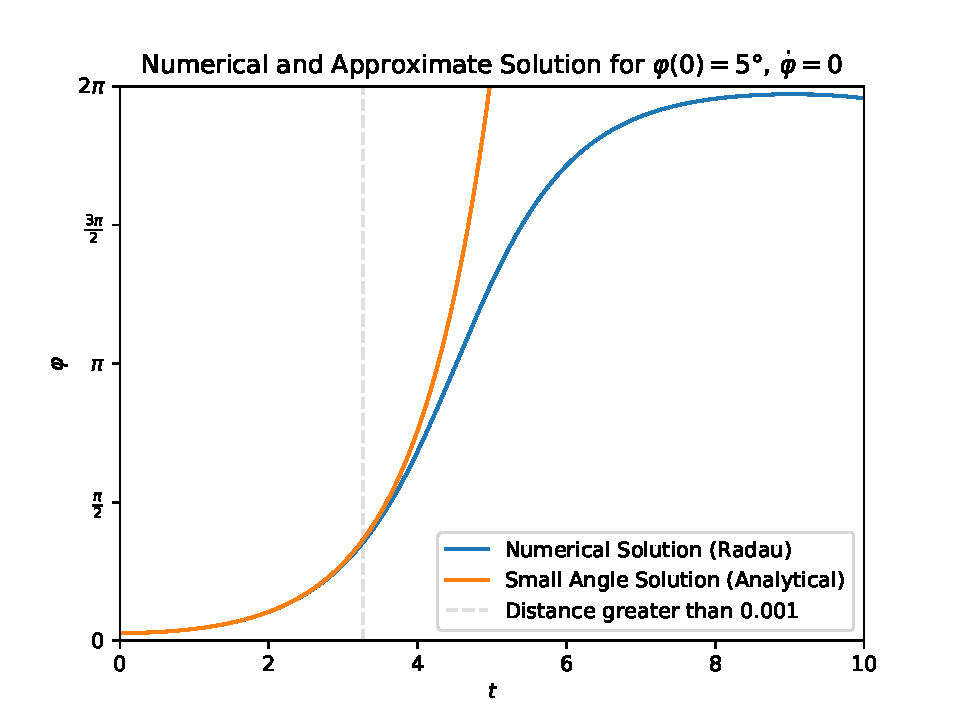
\includegraphics[width = \linewidth]{figures/introduction/generated/pendulum-motion-solutions}
					\caption{Trajectories of two solution strategies to the inverse pendulum, where the blue is a numerical solution of the actual motion of equation (solved using the Radau~IIA method~\cite[72]{hairerSolvingOrdinaryDifferential1996}) and the orange one is the analytically computed solution linearized \ac{ode}. The latter is linearized using small angle approximation. The dotted gray vertical line shows when the distance tolerance of \( \varepsilon = 10^{-3} \) is exceeded.}
				\end{subfigure}%
				~
				\begin{subfigure}[t]{0.5\linewidth}
					\centering
					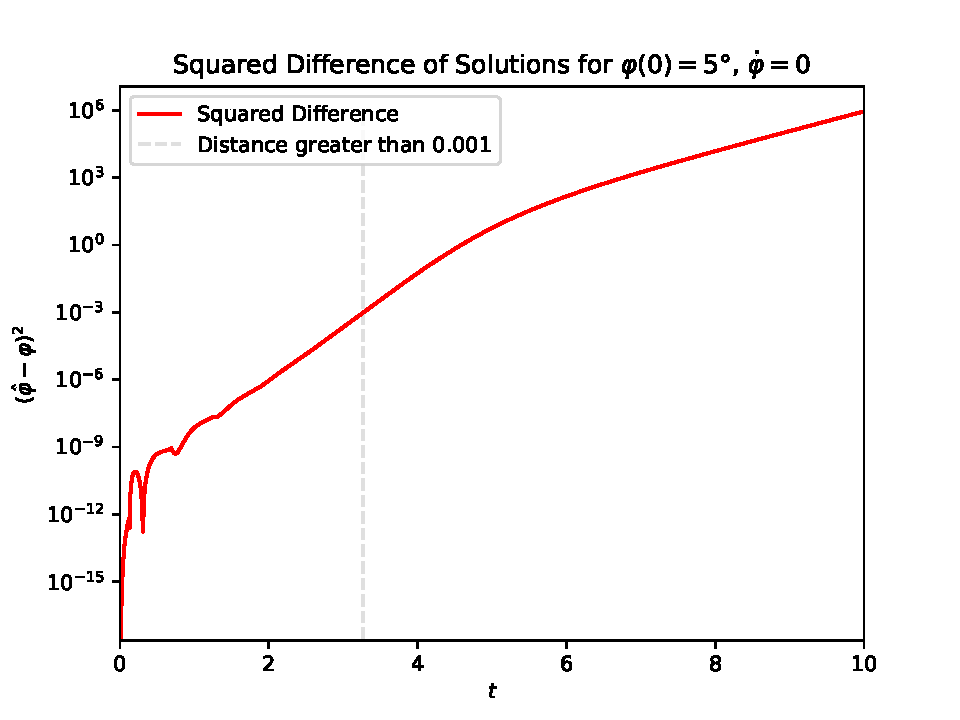
\includegraphics[width = \linewidth]{figures/introduction/generated/pendulum-motion-difference}
					\caption{Differences between the small angle approximation and the numerical solution of the \ac{ode}  The dotted gray vertical line shows when the distance tolerance of \( \varepsilon = 10^{-3} \) is exceeded.}
				\end{subfigure}
				\caption{Comparison of a numerical solution to the \ac{ode} of the inverse pendulum given in\eqref{eq:inversePendulum} and the analytical solution of the linearized \ac{ode} given in\eqref{eq:linearizedInversePendulum}. A tolerance value of \( \varepsilon = 10^{-3} \) is used to show when the both solutions diverge from each other.}
				\label{fig:inversePendulumApprox}
			\end{figure}
		% end
	% end
% end

	\chapter{Experiments}
	\label{c:experiments}

	\todo{Content}
% end

	\chapter{Results}
	\label{c:results}
	\IMRADlabel{results}

	\todo{Results: Content}
% end

	\chapter{Discussion}
	\label{c:discussion}
	\IMRADlabel{discussion}

	\todo{Discussion: Content}
% end

	\chapter{Outlook}
	\label{c:outlook}

	\todo{Outlook: Content}
% end


	\cleardoublepage
	\bibliography{literature/lit}
	\nocite{*}

	\cleardoublepage

	\appendix
	\chapter{Invent some nice chapter title} \todo{Chapter title.}
	\section{Solution of the Harmonic Oscillator}
		\label{app:harmonicOscillatorSolution}
	
		To solve the differential motion equation
		\begin{align*}
			m\ddot{x} = -kx
		\end{align*}
		of the harmonic oscillator given in~\autoref{subsec:harmonicOscillator}, we use the solution approach
		\begin{align*}
			x(t) = c e^{\lambda t} \qquad \dot{x}(t) = \lambda c e^{\lambda t} \qquad \ddot{x}(t) = \lambda^2 c e^{\lambda t}
		\end{align*}
		and insert it into the differential equation:
		\begin{align*}
			m\ddot{x} = -kx \quad\implies\quad
			m \lambda^2 c e^{\lambda t} = -k c e^{\lambda t} \quad\iff\quad
			m \lambda^2 = -k \quad\iff\quad
			\lambda = \pm \sqrt{-\frac{k}{m}}
		\end{align*}
		As both \(k\) and \(m\) are defined to be positive, we get the complex solutions:
		\begin{align*}
			x_1(t) = e^{i t \sqrt{k / m}} \qquad x_2(t) = e^{-i t \sqrt{k / m}}
		\end{align*}
		Due to the superposition principle, also \( x_1 + x_2 \) and \( x_1 - x_2 \) are solutions. Hence, we get two real solutions by using Euler's identity \( e^{\varphi i} = \cos(\varphi) + i \sin(\varphi) \):
		\begin{align*}
			x_1 + x_2
				&= e^{i t \sqrt{k / m}} + e^{-i t \sqrt{k / m}} \\
				&= \cos\Big(t \sqrt{k / m}\Big) + i \sin\Big(t \sqrt{k / m}\Big) + \cos\Big(t \sqrt{k / m}\Big) - i \sin\Big(t \sqrt{k / m}\Big) \\
				&= 2 \cos\Big(t \sqrt{k / m}\Big) \\
			x_1 - x_2
				&= e^{i \sqrt{k / m} t} - e^{-i t \sqrt{k / m}} \\
				&= \cos\Big(t \sqrt{k / m}\Big) i \sin\Big(t \sqrt{k / m}\Big) - \cos\Big(t \sqrt{k / m}\Big) + i \sin\Big(t \sqrt{k / m}\Big) \\
				&=  2i \sin\Big(t \sqrt{k / m}\Big)
		\end{align*}
		This yields the following general solution:
		\begin{align*}
			x(t) = c_1 \cos\Big(t \sqrt{k / m}\Big) + c_2 \sin\Big(t \sqrt{k / m}\Big),\quad c_1, c_2 \in \C
		\end{align*}
		As both Sine and Cosine are Sinusoidal, different \( c_1 \neq c_2 \) only lead to a phase shift. Thus we can also write the solution as
		\begin{align*}
			x(t) = A \cos\Big(t \sqrt{k / m} + \varphi\Big)
		\end{align*}
		with the amplitude \(A\) and the phase \(\varphi\).
	% end
% end

\end{document}
